\documentclass{beamer}

\usepackage{pdfpages}
\transduration{1}
\transfade

\usetheme{Madrid} % Du kannst z. B. auch Darmstadt, Berkeley, etc. probieren

\title{Visualisierung kinematischer Kennwerte}
\author{Philipp Mikos}
\date{\today}

\begin{document}


\frame{\titlepage}



\begin{frame}{Gliederung}
  \tableofcontents
\end{frame}



\section{Einleitung}
\begin{frame}{Einleitung}
  \begin{itemize}
    \setlength{\itemsep}{1em}
    \item Entwicklung von Framework zur Visualisierung kinematischer Kennwerte für die Lehre
    \item abstrakte mathematische Konzepte für Studenten schwierig zu durchdringen
    \item Besonderer Fokus: Rotation von Körpern
    \item Werkzeug für Lehrpersonen zum erstellen von Übungsszenarien
  \end{itemize}
\end{frame}


%Im Rahmen meiner Projektarbeit habe ich ein interaktives Framework entwickelt,
%das zur Visualisierung kinematischer Kennwerte gedacht ist – also Größen wie Position
%aber vor allem im kontext von diesem Projekt die Rotation.
%
%Ziel dieses Frameworks ist es, in der Lehre eingesetzt zu werden,
%zum Beispiel in Übungen oder Vorlesungen im Bereich der Robotik, um komplexe Bewegungsabläufe und Zusammenhänge greifbarer zu machen.
%
%Der Hintergrund ist der, dass es Studierenden oft schwer fällt,
%abstrakte mathematische Konzepte wie Transformationen im Raum wirklich zu verstehen.
%Begriffe wie Eulerwinkel oder Quaternionen bleiben häufig theoretisch und schwer vorstellbar.
%
%Ein besonderer Fokus meiner Arbeit liegt auf der Rotation von Körpern im Raum,
%da es eines der Ersten konzepte der Kinematik ist das im bereich der Robotik gelehrt wird
%
%insgesammt soll das Framework Lehrpersonen helfen, individuell anpassbare Übungsszenarien zu erstellen,
%in denen dann Studierende interaktiv mit Parametern arbeiten und experimentieren können und
%dadurch ein besseres und anwendungsnahes Verständnis für gewisse kinematische Konzepte entwickeln.




\section{Anforderungen}
\begin{frame}{Anforderungen}
  \begin{itemize}
    \setlength{\itemsep}{1em}
    \item Python-Schnittstelle
    \item Nutzung innerhalb von JupyterLab
    \item nach möglichkeit Visualisierung innerhalb von JupyterLab
    \item Transformationen von Körpern im Raum Visualisieren (insbesondere Rotation)
    \item Darstellungsmöglichkeiten (Euler, Matrix, Quaternionen)
  \end{itemize}
\end{frame}


\begin{frame}{Anforderungen}
  \begin{itemize}
    \setlength{\itemsep}{1em}
    \item keine lokale Installation
    \item komfortable erstellung und Anwendung von Übungsaufgaben
    \item Kompatibel mit Sympy
    \item einfache Bewegungsabläufe Radgetriebender Roboter
  \end{itemize}
\end{frame}


%Für die Entwicklung des Frameworks wurden mehrere Anforderungen festgelegt,
%die sich sowohl aus den didaktischen Zielen der Lehre als auch aus technischen und praktischen Überlegungen ergeben.
%
%Zunächst ist eine Python-Schnittstelle vorgesehen.
%Python ist eine moderne, weit verbreitete Programmiersprache mit einer klaren und gut lesbaren Syntax.
%Viele Studierende sind bereits mit ihr vertraut, was den Einstieg erleichtert und die Barriere zur Nutzung des Frameworks senkt.
%
%Ein weiterer zentraler Punkt ist die Integration in JupyterLab.
%Diese Umgebung wird bereits an der Fachhochschule Dortmund in den Robotik-Übungen verwendet und bietet eine plattformunabhängige,
%browserbasierte Arbeitsweise. Idealerweise sollen die Visualisierungen direkt innerhalb von JupyterLab ablaufen – also ohne separate Fenster oder zusätzliche Programme.
%Das fördert nicht nur die Portabilität, sondern vermeidet auch Hürden bei der Installation.
%
%Ein klarer Fokus liegt auf der Visualisierung von Transformationen, vor allem von Rotationen im dreidimensionalen Raum.
%Dazu sollen unterschiedliche Darstellungsformen unterstützt werden, wie Eulerwinkel, Rotationsmatrizen und Quaternionen.
%Diese Vielfalt ist wichtig, weil jede dieser Darstellungen ihre eigenen Vor- und Nachteile hat und in der Robotik unterschiedliche Anwendungsbereiche findet.
%
%Darüber hinaus soll das Framework kompatibel mit SymPy sein. SymPy ist eine symbolische Mathematikbibliothek in Python,
%die in vielen bestehenden Übungsnotebooks bereits verwendet wird. Eine gute Integration ermöglicht es, das neue Framework einfach in bestehende Materialien einzubinden.
%
%Ein weiterer Punkt ist, dass das Framework ohne lokale Installation funktionieren soll.
%
%Außerdem soll das Framework die einfache Erstellung und Durchführung von Übungsaufgaben unterstützen.
%Lehrende sollen damit unkompliziert Aufgaben formulieren und Lernende die Möglichkeit erhalten, interaktiv mit Parametern zu experimentieren.
%Zusätzlich sollen auch einfache Bewegungsabläufe radgetriebener Roboter abgebildet werden können, um kinematische Prinzipien greifbarer zu machen.






\section{Aufbau}
\begin{frame}{Aufbau}
  \begin{columns}
    \begin{column}{0.6\textwidth}
      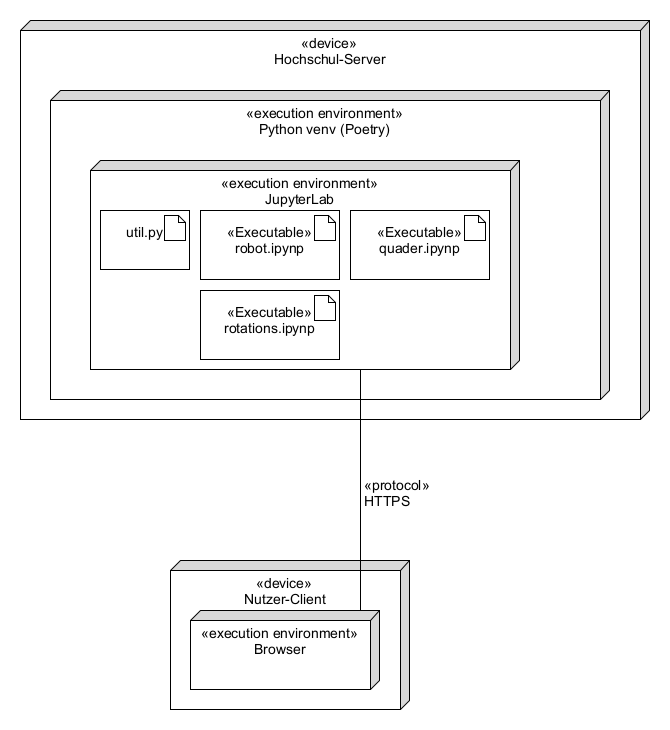
\includegraphics[width=\linewidth]{images/diagramme/komponentendiagramm.png}
    \end{column}
    \begin{column}{0.4\textwidth}
      \textbf{Weitere Abhängigkeiten:}\vspace{0.5em}
      \begin{itemize}
        \setlength{\itemsep}{1em}
        \item Numpy
        \item SymPy
        \item SciPy
        \item pythreejs(3D Rendering)
        \item ipywidgets(GUI-Elemente)
      \end{itemize}
    \end{column}
  \end{columns}
\end{frame}




\begin{frame}{Aufbau}
  \textbf{util.py:}\vspace{0.5em}
  \begin{itemize}
    \setlength{\itemsep}{1em}
    \item Zentrale Datei util.py mit Kern- und Hilfsfunktionen
    \item geometrische Transformationen und Umrechnung der Darstellungsformen von Rotationen
    \item Klasse Environment für konfigurierbare 3D-Szene mit Kamera, Licht und Gitter
    \item Funktion move() zur Simulation von Roboterbewegungen in der Ebene
  \end{itemize}
\end{frame}


\begin{frame}{Aufbau}
  \textbf{Beispiel-Notebooks: rotations.ipynb}\vspace{0.5em}
  \begin{itemize}
    \setlength{\itemsep}{1em}
    \item Würfel der interaktiv per GUI-Elementen transformiert werden kann
    \item Möglichkeiten des Frameworks veranschaulichen
    \item Grundtranfsformationen nachzuvollziehbar machen
  \end{itemize}
\end{frame}


\begin{frame}{Aufbau}
  \textbf{Beispiel-Notebooks: quader.ipynb}\vspace{0.5em}
  \begin{itemize}
    \setlength{\itemsep}{1em}
    \item Quader der anhand von Rotationsmatrizen rotiert werden soll
    \item Orientiert sich an einer Klausuraufgabe im Modul Robotik
    \item Visuelle Simulation der Rotationen
  \end{itemize}
\end{frame}


\begin{frame}{Aufbau}
  \textbf{Beispiel-Notebooks: robot.ipynb}\vspace{0.5em}
  \begin{itemize}
    \setlength{\itemsep}{1em}
    \item Veranschaulichung einer Steuerungsaufgabe
    \item Orientiert sich an einer Übungsaufgabe im Modul Robotik
    \item Nutzer kann beobachten ob der Roboter dem gewünschten Pfad folgt
  \end{itemize}
\end{frame}




%\section{Entwicklungsprozess}
%
%\begin{frame}{Entwicklungsprozess}
%  \textbf{Wahl der Rendering API:}\\
%  \textbf{OpenGL}\vspace{0.5em}
%  \begin{itemize}
%    \item Plattformunabhängig (Windows, macOS, Linux)
%    \item Bewährt in 3D-Grafik, CAD und Spieleentwicklung
%    \item Muss lokal installiert werden → höhere Systemanforderungen
%    \item Integration in Webanwendungen schwierig
%  \end{itemize}
%\end{frame}
%
%\begin{frame}{Entwicklungsprozess}
%  \textbf{Wahl der Rendering API:}\\
%  \textbf{WebGL}\vspace{0.5em}
%  \begin{itemize}
%    \item Läuft direkt im Browser ohne Zusatzsoftware
%    \item Plattformunabhängig durch HTML5-Kompatibilität
%    \item Gut geeignet für interaktive Webanwendungen
%    \item Relativ generisch → hoher Entwicklungsaufwand
%    \item Darstellung meist in separatem Browser-Tab
%  \end{itemize}
%\end{frame}
%
%\begin{frame}{Entwicklungsprozess}
%  \textbf{Wahl der Rendering API:}\\
%  \textbf{Babylon.js}\vspace{0.5em}
%  \begin{itemize}
%    \item 3D-Engine auf Basis von WebGL
%    \item Viele nicht benötigte Funktionen (z.B. Physik, Sound)
%    \item Schnelle Umsetzung komplexer Szenen
%    \item Kann unnötige Komplexität erzeugen
%    \item Darstellung ebenfalls in separatem Browser-Tab
%  \end{itemize}
%\end{frame}
%
%\begin{frame}{Entwicklungsprozess}
%  \textbf{Wahl der Rendering API:}\\
%  \textbf{Three.js}\vspace{0.5em}
%  \begin{itemize}
%    \item Basiert ebenfalls auf WebGL
%    \item Gute Balance zwischen Kontrolle und Abstraktion
%    \item Flexibel, leichtgewichtig und erweiterbar
%    \item Ideal für sich entwickelnde Anforderungen
%    \item Darstellung in separatem Browser-Tab bleibt Einschränkung
%  \end{itemize}
%\end{frame}
%
%%prototypen vorstellen
%
%\begin{frame}{Entwicklungsprozess}
%  \textbf{Numpy als Mathematik-Library:}\vspace{0.5em}
%  \begin{itemize}
%    \item Bessere Performance als SymPy
%    \item symbolische Verarbeitung nicht erforderlich
%    \item Kompatibilität mit SymPy durch Umwandlungen dennoch gegeben
%  \end{itemize}
%\end{frame}
%
%
%\begin{frame}{Entwicklungsprozess}
%  \textbf{Environment-Klasse}\vspace{0.5em}
%  \begin{itemize}
%    \item Wiederkehrende elemente in den Beispiel-Notebooks in einer Klasse zusammengefasst
%    \item Kapselt Erstellung und Verwaltung einer 3D Szene (Kamera, Lichtquelle, Gitter, Achsen) und GUI-Elemente
%    \item einfaches Hinzuzufügen von GUI- und Szenen-Elementen
%  \end{itemize}
%\end{frame}


\section{Evaluation}
\begin{frame}{Evaluation}
  \begin{itemize}
    \setlength{\itemsep}{1em}
    \item Erfolgreiche Integration in JupyterLab: einfache Nutzung und direkte Visualisierung
    \item Unterstützung verschiedener Rotationsdarstellungen inkl. Umrechnungen
    \item Simulation radgetriebener Roboter über move()-Funktion realisiert
    \item Kompatibilität mit SymPy sichergestellt
    \item Zentrale Anforderungen erfüllt. Grundlage für spätere Erweiterungen geschaffen
  \end{itemize}
\end{frame}




\section{Ausblick auf die Bachelorarbeit}
\begin{frame}{Ausblick auf die Bachelorarbeit}
  \begin{itemize}
    \setlength{\itemsep}{1em}
    \item Deployment auf den JupyterLab-Servern der FH Dortmund
    \item Erweiterungen um Stationäre Robobter
    \item vorwärts- und rückwärts-Transformation
    
  \end{itemize}
\end{frame}


\begin{frame}{}
  \begin{center}
    \textbf{\huge Vielen Dank für Ihre Aufmerksamkeit!}  
  \end{center}
  
\end{frame}





\end{document}
